\documentclass[a4paper]{proc}
\title{Fitting SARMA Models Onto Activity and Skin Temperature Time Series Data}
\author{Sherman Ip$\qquad$March 10, 2016}

\usepackage{amsmath}
\usepackage{amsfonts}
\usepackage{amssymb}
\usepackage{graphicx}
\usepackage{subcaption}
\usepackage{caption}

\DeclareMathOperator{\expectation}{E}

\newcommand{\euler}{\mathrm{e}}
\newcommand{\diff}{\mathrm{d}}
\newcommand{\T}{^\textup{T}}
\newcommand{\vect}[1]{\mathbf{#1}}
\newcommand{\vectGreek}[1]{\boldsymbol{#1}}
\newcommand{\matr}[1]{\mathsf{#1}}
\newcommand{\dotdotdot}{\vphantom{.}_{\cdots}}
\newcommand{\backshift}{\widehat{B}}

\begin{document}

\maketitle

\begin{abstract}
Abstract
\end{abstract}

\section{Introduction}
Suppose a time series $\{Y_1,Y_2,\dotdotdot,Y_T\}$ was observed and, without lost of generality, has zero mean. An ARMA$(p,q)$ model can be fitted which has the form
\begin{equation}
Y_t = \sum_{i=1}^{p} \phi_i Y_{t-i} + \epsilon_t - \sum_{j=1}^{q} \theta_{j} \epsilon_{t-j}
\label{eq:ARMA}
\end{equation}
where $\epsilon_t$ are some i.i.d.~distributed noise with zero mean and variance $\sigma^2$.

By using the backshift operator $\backshift$ where
\begin{align}
\backshift Y_t &= Y_{t-1} \\
\backshift \epsilon_t &= \epsilon_{t-1} \ ,
\end{align}
Equation \eqref{eq:ARMA} can be expressed as
\begin{equation}
Y_t = \sum_{i=1}^{p} \phi_i \backshift Y_{t} + \epsilon_t - \sum_{j=1}^{q} \theta_{j} \backshift \epsilon_{t}
\end{equation}
which can be rearranged to
\begin{equation}
\theta\left(\backshift\right)Y_t=\phi\left(\backshift\right)\epsilon_t
\end{equation}
where
\begin{align}
\phi(x)&=1-\sum_{i=1}^{p} \phi_i x \\
\theta(x)&=1-\sum_{i=1}^{q} \theta_i x
\end{align}
are called the AR and MA characteristic equations respectively.

Seasonality, of lag $s$, can be considered by including the AR and MA seasonal characteristic equation, $\Phi(x)$ and $\Theta(x)$ respectively, where
\begin{align}
\Phi(x) &= 1 - \sum_{i=1}^P \Phi_i x^{is} \\
\Theta(x) &= 1 - \sum_{j=1}^Q \Theta_j x^{js} \ .
\end{align}
The SARMA$(p,q)\times(P,Q)_s$ model uses the seasonal characteristic equation where the model has the form
\begin{equation}
\phi\left(\backshift\right)\Phi\left(\backshift\right)Y_t
=
\theta\left(\backshift\right)\Theta\left(\backshift\right)\epsilon_t
\end{equation}

Assuming the noise is Normally distributed, the maximum likelihood can be used to estimate the SARMA parameters: $\phi_1,\dotdotdot,\phi_p,\theta_1,\dotdotdot,\theta_q,\Phi_1,\dotdotdot\Phi_P,\Theta_1,\dotdotdot,\Theta_Q$. The assumption of Normal i.i.d.~noise can be checked by investigating the residuals of fitting the SARMA model onto the data.

The objective was to fit SARMA onto activity and skin temperature time series data and see how they perform.

\section{Methods}
Selecting $p,q,P,Q,s$ to fit the SARMA model, onto the time series data, is troublesome because it involves investigating 5 parameters.

$s$ was selected and fixed to be 24 hours because it was observed, by inspection, that there may be a cyclic behaviour, with a period of 24 hours, in the time series.

The Akaike information criterion (AIC) and Bayesian information criterion (BIC) was used to select which $p,q,P,Q$ to fit the SARMA model onto the data. The information criterions have the form
\begin{align}
\textup{AIC}&=T\ln{\widehat{\sigma}^2}+(p+q+P+Q)2\\
\textup{BIC}&=T\ln{\widehat{\sigma}^2}+(p+q+P+Q)\ln{T}
\end{align}
where $\widehat{\sigma}^2$ is the estimated variance of the residuals. Firstly, ARMA$(p,q)$ models were fitted for $p=0,1,\dotdotdot,5$ and $q=0,1,\dotdotdot,5$. The $p,q$ pair which minimises an information criterion was selected and fixed. Secondly, SARMA$(p,q)\times(P,Q)_s$ models were fitted for $P=0,1,2$ and $Q=0,1,2$. The $P,Q$ pair was selected which minimises an information criterion. MATLAB \emph{regARMA} was used to fit the SARMA model onto the data.

The model was tested by fitting the SARMA model, using the AIC/BIC procedure, onto the first 3 days of the data. The model was then extrapolated to do a 24 hour forecast. Such a forecast was then compared with the actual data using the mean squared error (and the logarithmic scoring). That is suppose $\{\widehat{Y}_{T+1},\widehat{Y}_{T+2},\dotdotdot,\widehat{Y}_{T+h}\}$ was the forecast of $\{{Y}_{T+1},{Y}_{T+2},\dotdotdot,{Y}_{T+h}\}$, then the mean squared error (MSE) was calculated using
\begin{equation}
\textup{MSE} = \frac{\sum_{k=1}^{h}\left(\widehat{Y}_{T+k}-Y_{T+k}\right)^2}{h} \ .
\end{equation}

The forecast error, $\{\widehat{e}_{T+1},\widehat{e}_{T+2},\dotdotdot,\widehat{e}_{T+h}\}$, was obtained and used to estimate approximately the error in the MSE using the Delta method given as
\begin{equation}
\sigma_{\textup{MSE}} = \frac{2}{h}\sqrt{\sum_{k=1}^{h}\left(\widehat{Y}_{T+k}-Y_{T+k}\right)^2\left(\widehat{e}_{T+k}\right)^2} \ .
\end{equation}

\section{Results}
SARMA$(p,q)\times(P,Q)_{24}$ models were fitted onto the 8 time series data independently. As an example, Figure \ref{fig:sarmafit} shows the selected SARMA model, using AIC, being fitted onto the time series data of subject 8. The model was extrapolated to do a 24 hour forecast.

It was observed that the forecast error on the activity time series blew up in the order of $\sim 10^2$. A forecast with such an error is practically useless thus it was considered that the SARMA model did not fit well with the activity time series.

The forecast error on the temperature time series was sensible, for example in Figure \ref{fig:sarmafit}.

\begin{table}
\begin{center}
\begin{tabular}{ cccccc } 
 Data & p & q & P & Q & MSE\\
  \hline
 Temp2 & 4 & 2 & 2 & 2 & $1.1\pm0.2$\\
 Temp8 & 2 & 5 & 2 & 0 & $1.5\pm0.1$\\
 Temp24& 5 & 4 & 2 & 0 & $0.54\pm0.06$\\
 Temp26& 2 & 4 & 2 & 0 & $0.69\pm0.06$\\
\end{tabular}
\end{center}
\caption{Hello.}
\label{table:AIC}
\end{table}

\begin{table}
\begin{center}
\begin{tabular}{ cccccc } 
 Data & p & q & P & Q & MSE\\
  \hline
 Temp2 & 1 & 0 & 2 & 2 & $1.1\pm0.2$\\
 Temp8 & 2 & 1 & 2 & 0 & $1.4\pm0.1$\\
 Temp24& 2 & 4 & 1 & 1 & $0.28\pm0.03$\\
 Temp26& 2 & 0 & 2 & 0 & $0.72\pm0.07$\\
\end{tabular}
\end{center}
\caption{Hello.}
\label{table:BIC}
\end{table}

\begin{figure*}
    \begin{subfigure}[b]{\textwidth}
        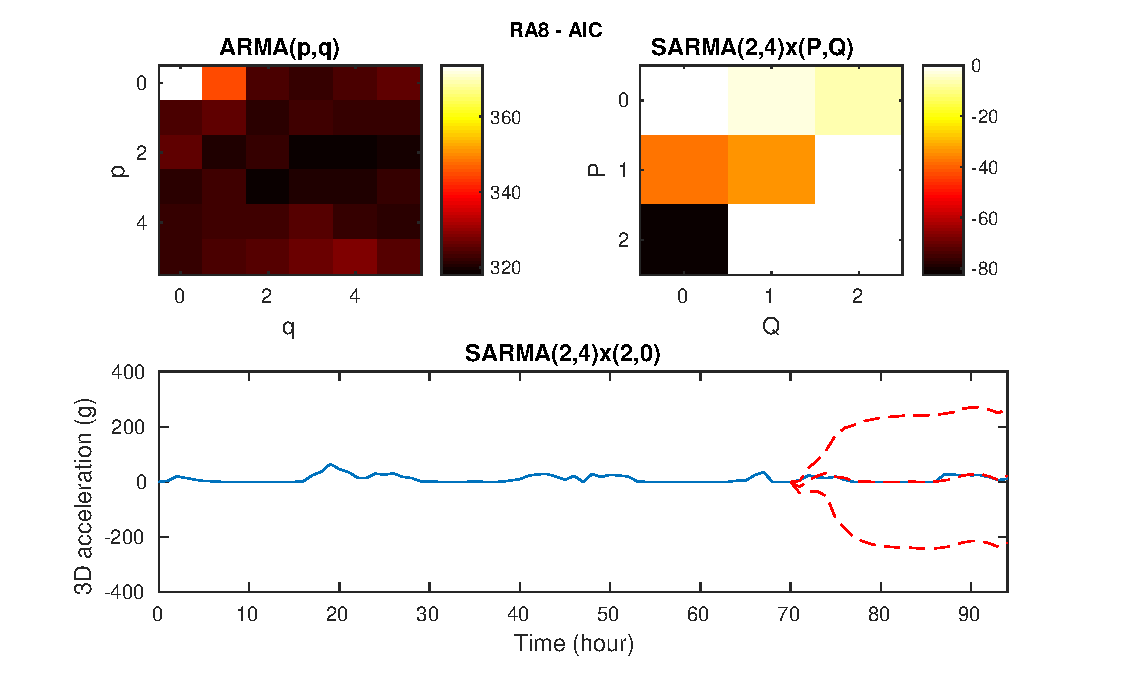
\includegraphics[width=\textwidth]{aic_ra_8.eps}
        \caption{Activity}
    \end{subfigure}
    \begin{subfigure}[b]{\textwidth}
        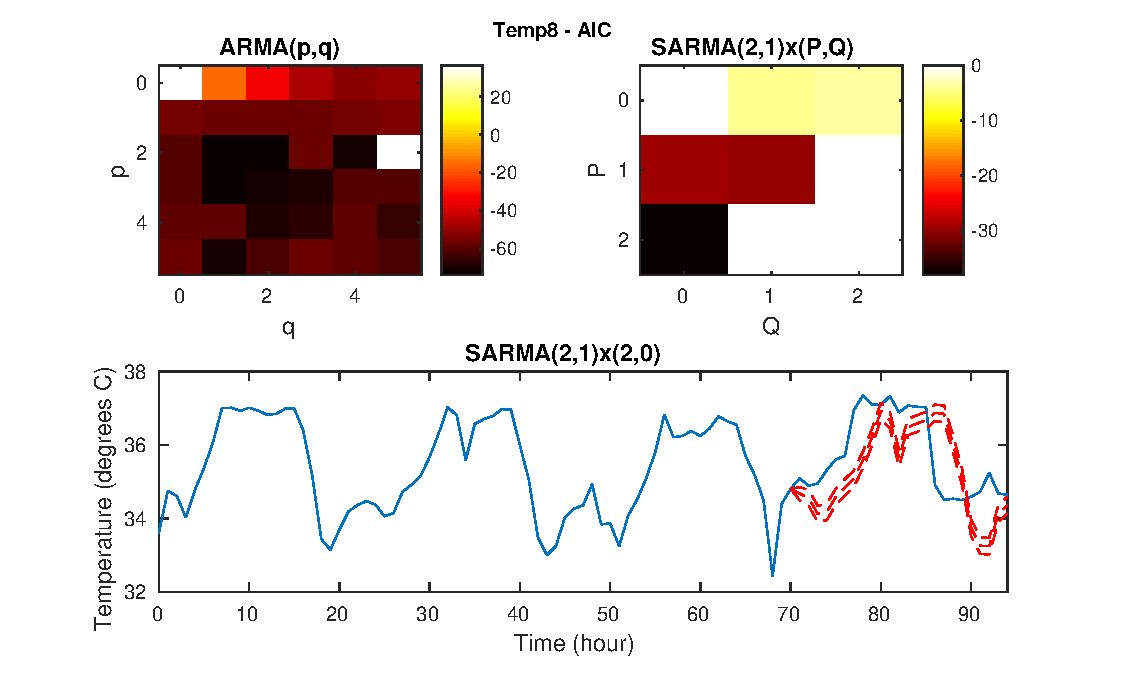
\includegraphics[width=\textwidth]{aic_temp_8.eps}
        \caption{Skin Temperature}
    \end{subfigure}
    \caption{hello}
    \label{fig:sarmafit}
\end{figure*}

\end{document}
